%%%%%%%%%%%%%%%%%%%%%%%%%%%%%%%%%%%%%%%%%%%%%%%%%%%%%%%%%%%%%%%%%%%%%%%%%%%%%%%%%%%%%%%%%%%%%%%%%%%%

\chapter{Properties of individual molecular outflows in \ngc253}
\chaptermark{individual molecular outflows}
\label{chapter: outflow catalog}

%%%%%%%%%%%%%%%%%%%%%%%%%%%%%%%%%%%%%%%%%%%%%%%%%%%%%%%%%%%%%%%%%%%%%%%%%%%%%%%%%%%%%%%%%%%%%%%%%%%%

\begin{papernote}
The work presented in this chapter was carried out alongside the work published in \citet[; Chapter~\ref{chapter: outflow}]{2019ApJ...881...43K} but ultimately was chosen to not be included in that publication.
\end{papernote}


%%%%%%%%%%%%%%%%%%%%%%%%%%%%%%%%%%%%%%%%%%%%%%%%%%%%%%%%%%%%%%%%%%%%%%%%%%%%%%%%%%%%%%%%%%%%%%%%%%%%
%%%%%%%%%%%%%%%%%%%%%%%%%%%%%%%%%%%%%%%%%%%%%%%%%%%%%%%%%%%%%%%%%%%%%%%%%%%%%%%%%%%%%%%%%%%%%%%%%%%%

\section{Introduction}\label{outflow catalog: section: introduction}

It is known for several years now that \ngc253 hosts a molecular outflow \citep{2006ApJ...636..685S,2013Natur.499..450B}. In the previous chapter, we discuss what can be learned from a global view on the molecular outflow at low resolutions at scales of dozens of parsecs.
Only with the high spatial resolution at simultaneously high sensitivity achievable with ALMA in the recent years, it has become possible to resolve structures (streamers) within the outflow \citep{2017ApJ...835..265W}. 
A comparison between low and high resolution CO data in Chapter~\ref{chapter: outflow} shows that a considerable fraction of $\sim50$\% of the CO emission is located in localized structures.
Figure~\ref{outflow catalog: figure: false color} highlights said structures by colorcoding the gas velocity. %in false colors.
Alongside the projected molecular disk, streamers are easily spotted in Figure~\ref{outflow catalog: figure: false color} by their mismatching color which indicates that they are at a different velocity than the local disk velocity.
Immediately visible from Figure~\ref{outflow catalog: figure: false color}, the streamers vary in orientation or velocity at the same projected position. In this chapter, we will catalog the streamers to examine these and other properties to answer the question how a typical streamer in the molecular outflow is structured.

In order to also quantify outflow properties in the highest possible detail, it is necessary to manually identify potentially outflowing structures since automated methods still do not reach the human ability to identify structures.
Manual identification introduces an observer bias but on the other hand better utilizes the high resolution available, so it is complementary to the large scale approach presented in Chapter~\ref{chapter: outflow}.

\begin{figure*}[t]
	\centering
	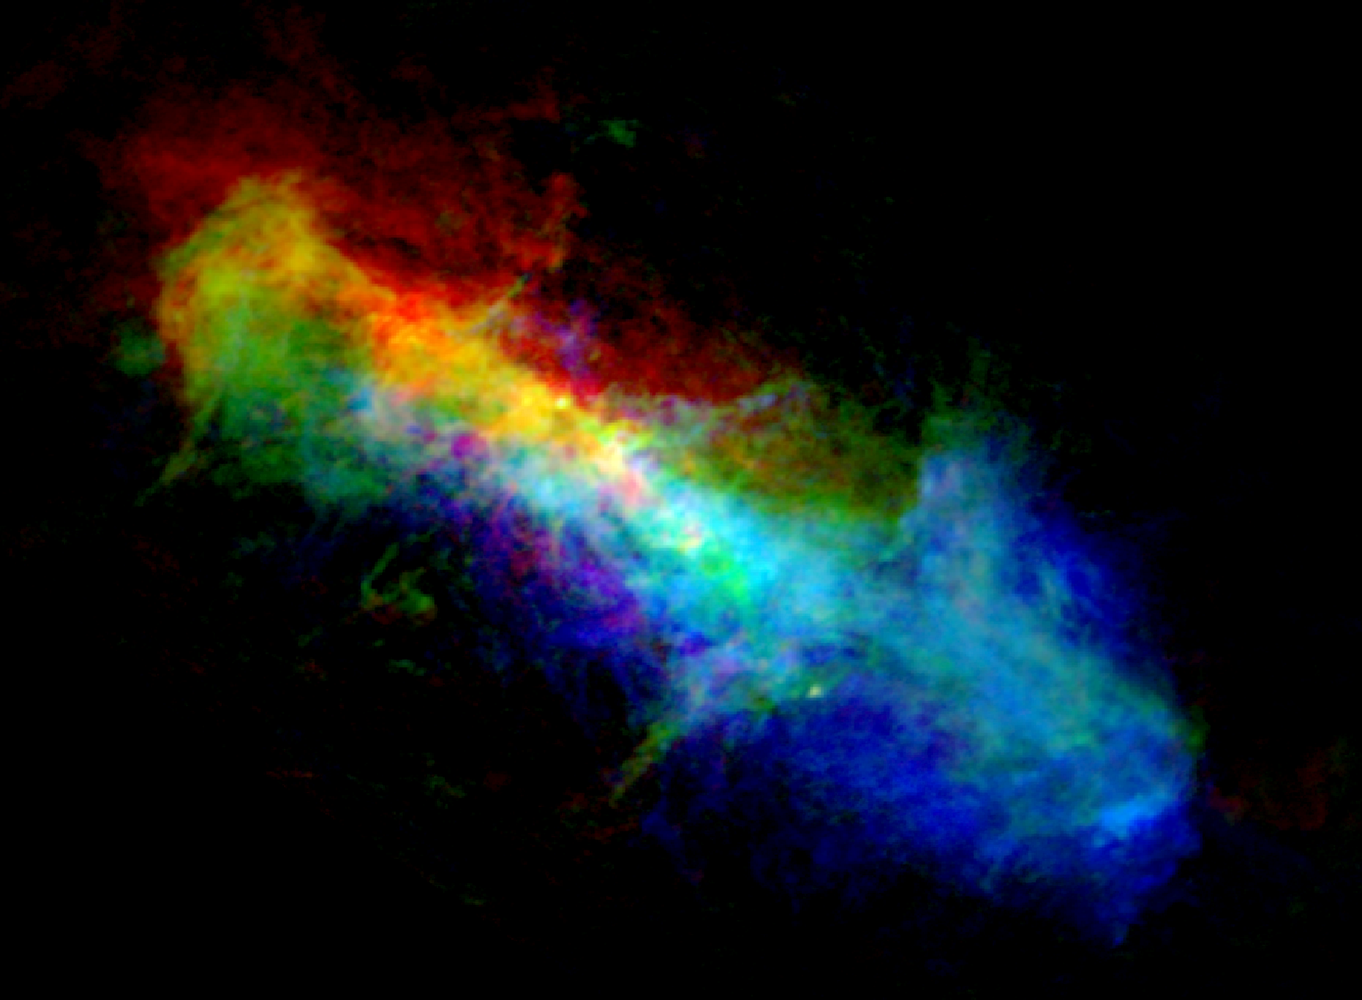
\includegraphics[width=\linewidth]{images/chapters/papers/outflow_catalog/CO32_false_color.png}
	\caption[Colorcoded velocity structure]{\co32 emission in the central $\sim1$\,kpc of \ngc253 colorcoded by velocity. Gas at the systemic velocity ($230-270$\,\kms) is shown in green while the redshifted ($\GTR 270$\,\kms) and blueshifted ($\LESS 230$\,\kms) emission in shown in the respective color. This choice of velocity intervals highlights the disturbed velocity field and prominently features the molecular streamers perpendicular to the projected disk.
	Note that this image shows the full dataset as presented in Chapter~\ref{chapter: outflow} at 2.5\,pc resolution while the analysis in this chapter is based on earlier observations with 7.5\,pc resolution.
	}\label{outflow catalog: figure: false color}
\end{figure*}


%%%%%%%%%%%%%%%%%%%%%%%%%%%%%%%%%%%%%%%%%%%%%%%%%%%%%%%%%%%%%%%%%%%%%%%%%%%%%%%%%%%%%%%%%%%%%%%%%%%%
%%%%%%%%%%%%%%%%%%%%%%%%%%%%%%%%%%%%%%%%%%%%%%%%%%%%%%%%%%%%%%%%%%%%%%%%%%%%%%%%%%%%%%%%%%%%%%%%%%%%

\section{Data reduction and imaging}

Obtaining a full ALMA dataset including multiple array configurations and total power data requires a substantial amount of time. The analysis presented in this chapter was thus conducted while the observation program was still ongoing and the highest resolution data (12\,m extended configuration) as well as the single dish data (total power array) was not yet observed. The following data therefore represent a subset of the complete dataset shown in Chapter~\ref{chapter: outflow}.

The observational setup is the same as for the full dataset with 7.6\,GHz spectral coverage (LSB: $342.0-345.8$\,GHz, USB: $353.9-357.7$\,GHz) in 976.6\,kHz channels (corresponding to 0.8\,\kms) and a linear four pointing mosaic covering the central $\sim750$\,pc of \ngc253. 
The observations were carried out in the compact configuration of the 12\,m array (baselines $15.1-83.5$\,m) in mid 2016 (12-Apr-2016, 23-Apr-2016, 17-Jun-2016, 27-Jun-2016) with typically 36~antennas and a total 2.6\,h on-source observation time.
The calibrators are: J0006-0623 (bandpass); J0038-2459 (complex gain); the asteroid Pallas (absolute flux density); J0104-2416, J0106-2718 (both WVR). The visibilities are calibrated using the ALMA cycle 3 pipeline in \casa 4.6.0 and the delivered calibration script.

In order to image the spectral lines, the continuum is subtracted using a first order polynomial fitted to the channels that do not contain strong spectral lines. At this resolution, we detect $\sim21$ spectral lines aside from the four strong lines \co32, \hcn, \hco and \cs. However, these lines are weak and only detected towards the central continuum sources (cf. Chapter~\ref{chapter: SSCs}) which is why they do not affect the overall continuum fit and subtraction.

For obtaining the final images and data cubes, we employ a multi-stage masking and \clean process. This ensures that \clean converges reliably and confines \clean masks to regions of real emission. We run an initial multi-scale \clean to $5\sigma$ with the rms noise level $\sigma = 75$\,mK of the dirty image without any spatial constraints. A mask that contains all pixels at $\GTR 2.5\sigma$ and enlarged to also include the surrounding $\sim0.5$\arcsec defines the \clean mask for the final multi-scale \clean run. In this final run (scales [0,3,9,27] with pixel size 0.1\arcsec), we clean the detected emission to $2.5\sigma$. 
All imaging tasks were carried out in \casa 4.6.0 with natural weighting and 2\,\kms channel width, imaging 500\kms centered on the redshifted ($v_\mathrm{sys} = 250$\,\kms) rest frequency. 
The noise in the final image is 75\,mK (1.35\,m\jybeam) in a 2.0\,\kms channel. The beam size is $0.48\arcsec \times 0.38\arcsec$ which corresponds to 8.1\,pc $\times$ 6.4\,pc at the distance of NGC 253.


\begin{table}
    \centering
    \begin{threeparttable}
    	\caption{Observation and image parameters.
    	\label{outflow catalog: table: image parameters}}
    % 	\footnotesize
        \begin{tabular}{ll}
            \toprule
            \ngc253                                                         \\
            \midrule
            distance            & 3.5\,Mpc                                  \\
            $v_\mathrm{sys}$    & 250\,\kms                                 \\ 
            \midrule
            Observations                                                    \\
            \midrule
        	project code        & 2015.1.00274.S                            \\
        	configuration       & 12\,m array, compact                      \\
        	baselines           & $15.1-83.5$\,m                            \\
        	spectral coverage   & $342.0-345.8$\,GHz                        \\
        	                    & $353.9-357.7$\,GHz                        \\
        	\midrule
        	Imaging                                                         \\
        	\midrule
        	beam                & $0.48\arcsec \times 0.38\arcsec$          \\
        	                    & 8.1\,pc $\times$ 6.4\,pc                  \\
        	channel width       & 2.0\,\kms                                 \\
        	rms noise           & 75\,mK                                    \\
        	                    & 1.35\,m\jybeam                            \\
            \bottomrule
        \end{tabular}
    \end{threeparttable}
\end{table}


%%%%%%%%%%%%%%%%%%%%%%%%%%%%%%%%%%%%%%%%%%%%%%%%%%%%%%%%%%%%%%%%%%%%%%%%%%%%%%%%%%%%%%%%%%%%%%%%%%%%
%%%%%%%%%%%%%%%%%%%%%%%%%%%%%%%%%%%%%%%%%%%%%%%%%%%%%%%%%%%%%%%%%%%%%%%%%%%%%%%%%%%%%%%%%%%%%%%%%%%%

\section{Construction on an outflow catalog}\label{outflow catalog: section: construction}

The identification of outflow candidates is based on visual inspection and their physical properties:
apparent filaments of high aspect ratio visible in channel maps (Figure~\ref{outflow: figure: CO channel map}) and integrated intensity (Figure~\ref{outflow: figure: CO moment maps}a) as well as higher velocity dispersion than the surrounding due to blending of a second kinematic component (Figs.~\ref{outflow: figure: CO moment maps}c, \ref{outflow: figure: co pV}). Potential outflows are those structures that contain gas at velocities outside the range of the rotating disk (cf. Section~\ref{outflow: section: disk separation}).

We identify 11 outflow candidates that are marked with approximate length and position angle in Figure~\ref{outflow catalog: figure: outflow catalog}. Names (o1 to o11) are assigned clockwise starting at the most prominent outflow, the south-west (SW) streamer. Annotated pV diagrams for the outflow candidates are given in Figure~\ref{outflow catalog: figure: outflow catalog pV}.
There is significant overlap with the ``features consistent with outflowing gas'' defined in \co21 by \citet{2018ApJ...867..111Z}: the SW streamer (o1 in this work) corresponds to SWS $1-3$ in Zschaechner et al. and our outflow candidates o3, o4, o8, o7 and o9/o10 correspond to the points OF$1-5$, respectively.

For each outflow candidate, we generate a mask in position-position-velocity (ppV) space with an intensity cut at $5\sigma$ rms noise level. For a projection of this mask onto the outflow major axis/velocity plane, see the shaded regions in Figure~\ref{outflow catalog: figure: outflow catalog pV}.


\paragraph{Size}
For each of these outflow candidates, we estimate the projected length (width) as the greatest extent along the long (short) dimension of the candidate. The projected extent is derived from the integrated intensity map of the $5\sigma$ (375\,mK) masked outflow candidate.

\paragraph{Orientation}
Orientation denotes the position angle (PA) of the outflow candidate's long axis (length) in the convention north to east. For reference, the molecular disk in \ngc253 is oriented at $\mathrm{PA_{maj}} = 55^\circ$ and $\mathrm{PA_{min}} = 145^\circ$ for the major and minor axis, respectively.

\paragraph{Mass}
We derive the molecular gas mass of the outflow candidates from the ppV $5\sigma$ masked integrated intensity. Following \citet{2013ARA&A..51..207B}, we adopt a starburst conversion factor X$_{CO} = 0.5 \times 10^{20}$\,\sqcm\,K$^{-1}$\,\kms and correct for the contribution of helium.

\paragraph{Velocity information}
Similar to the spatial extent of the outflow candidates, it is possible to estimate the velocity ranges over which the candidates can be traced. This is done in pV diagrams calculated from the data cube masked at the $5\sigma$-level.

We measure the velocity dispersion as the mean velocity dispersion (intensity-weighted second moment) over the ppV mask defining each outflow candidate.

Within the masked pV diagram of each candidate, we fit the median velocity (red line in Figure~\ref{outflow catalog: figure: outflow catalog pV}) with a first order polynomial (dashed red line in Figure~\ref{outflow catalog: figure: outflow catalog pV}) within the outflow mask.
For o8, we restrict the velocity gradient estimation to the linear part, ignoring the turn-over of the median velocity at the tip of this structure (offset $\GTR 0$\arcsec).
In o9 and o10, the pV structure splits into two arms affecting the estimation of median velocity, velocity dispersion and velocity gradient. In both cases, we follow the upper arm that connects linearly to the disk.
Note that these estimates are \emph{projected velocity gradients} that do not take geometrical effects like inclination and outflow cone angle into account.
\citet{2017ApJ...835..265W} demonstrated for the SW streamer that projected velocity gradients do not necessarily translate to velocity gradients in 3D space.

We also try to estimate the velocity of the disk gas at the position of the outflow candidate, i.e. within the shaded region in Figure~\ref{outflow catalog: figure: outflow catalog}, in order to interpret the observed gradients with respect to the local disk velocity.
This estimate must not be biased towards an outflow if the ratio of outflow to disk intensity is high (e.g. o1) to obtain a meaningful estimate of the disk velocity.
It also needs to be robust against sub-optimal choices of outflow masks, i.e. should not rely solely on the outflow masks.
These requirements are met by using the median velocity of a high SNR image cube (masked arbitrarily at $80\sigma$) where the ppV space covered by the fainter outflow candidates is masked out.
The velocity model obtained in Chapter~\ref{outflow: section: disk separation} is not a useful reference here because on the small spatial scales of the outflow candidates the local disk velocity can deviate from the large-scale model.

\paragraph{Outflow launching sites}
In trying to estimate the launching sites of the outflow candidates, two launching mechanisms need to be considered as they differ in pV structure:
If molecular gas is directly expelled by energetic processes like supernovae or forms in a directly ejected outflow of hot ionized gas through condensation, the observed molecular outflow has an initial velocity $v_0 \GTR 0$. Theoretical models suggest SN gas ejection velocities of $\sim 100$\,\kms creating a strong discontinuity between outflow and disk gas from which it is ejected. Simulations of large scale outflows like e.g. \citet{2018ApJ...853..173K} show ejection velocities $\GTR 20$\,\kms which would also be visible in our pV diagrams.
If ionized or neutral outflows launch molecular gas by entrainment at the edge or within an ionized/neutral outflow, no initial velocity should be observed ($v_0 = 0$) and the molecular gas should be more gradually accelerated.
The first picture causes the problem of launching dense molecular gas by energetic processes without destroying the gas (dissociating molecules, ionization).
In \ngc253, the outflow phases follow a stratification of an inner ionized, fast outflow, surrounded by a neutral outflow cone and another cone of molecular outflow \citep{2015ApJ...801...63M}. The gradual launching process with $v_0 = 0$, thus seems to be more likely. Also, the pV diagrams in Figure~\ref{outflow catalog: figure: outflow catalog pV} do not show a significant velocity offset but the outflow candidates seem to connect smoothly to the disk in most cases.

In o1, o2, o3, o4, o7, o8, o9 and o10, we can trace back the outflow candidates in ppV space to where they intersect the local disk with $v_0 =0$. Under the assumption of strictly linear movement, i.e. linear velocity gradient and linear movement in the plane of the sky, the outflow candidates would originate from these points which is a first estimate of the launching site. Figures~\ref{outflow catalog: figure: outflow catalog} and \ref{outflow catalog: figure: outflow catalog pV} indicate the launching sites with red crosses. Physically, this launching site estimation corresponds to outflows that are smoothly accelerated away from their launching site in a straight line.

\paragraph{Kinetic energy}
With the kinematic structure and masses, it is possible to estimate the kinetic energy for the outflow candidates in two ways.
The internal kinetic energy measured by the velocity dispersion of the outflow candidate can be calculated given the ppV masks and estimated as $\frac{m}{2} \sigma^2$. This energy estimate is referred to as $\mathrm{E}_{kin,disp}$ in Table~\ref{outflow catalog: table: outflow catalog}.
If a launching site can be reconstructed it is also possible to calculate the bulk kinetic energy of the outflowing gas relative to that zero point by integrating along the outflow candidate $\mathrm{E}_{kin,launch} = \int \frac{m}{2} \left( v_i - v_{launch} \right)^2 \mathrm{d}v_i$.

\paragraph{Dynamical age}
The dynamical age of an outflow can be estimated by the time it took the tip to reach its current position. As before, the velocity gradient $v'$ in pV space is taken to be constant as was fitted to the median velocities.
The derivation of meaningful time scales require the following assumptions on the 3D structure.
As the simplest assumption, we take all outflow candidates to lie perpendicular to the disk because the true angle cannot be reconstructed and most candidates are found to lie roughly perpendicular to the projected disk (see the discussion below). The projected quantities offset $x_{proj}$, radial velocity $v_{rad}$ and velocity gradient $v'$ can then be deprojected when taking inclination $i$ into account:

\begin{eqnarray}
	x_{3D} &=& \frac{x_{proj}}{\sin i} \nonumber\\
	v_{3D} &=& \frac{v_{rad}}{\cos i} \nonumber\\
	v'_{3D} &=& \frac{\mathrm{d}v_{rad}}{\mathrm{d}x_{proj}} = v'_{proj} \times \tan i \nonumber
\end{eqnarray}

The dynamical age is given by the distance $x_{3D}$ between base and tip of an outflow candidate and the fitted velocity gradient. The base is either the launching site or the inner edge of the outflow mask if no launching site could be reconstructed.

\begin{displaymath}
	\mathrm{t}_{dyn}\,[\mathrm{Myr}] = 0.98 \times \frac{\ln \left( x_{3D}\,[\mathrm{pc}] \right)}{v'_{3D}\,[\mathrm{km}\,\mathrm{s}^{-1}\,\mathrm{pc}^{-1}]}
\end{displaymath}

The prefactor 0.98 handles the unit conversions.

\begin{figure}[t]
	\centering
	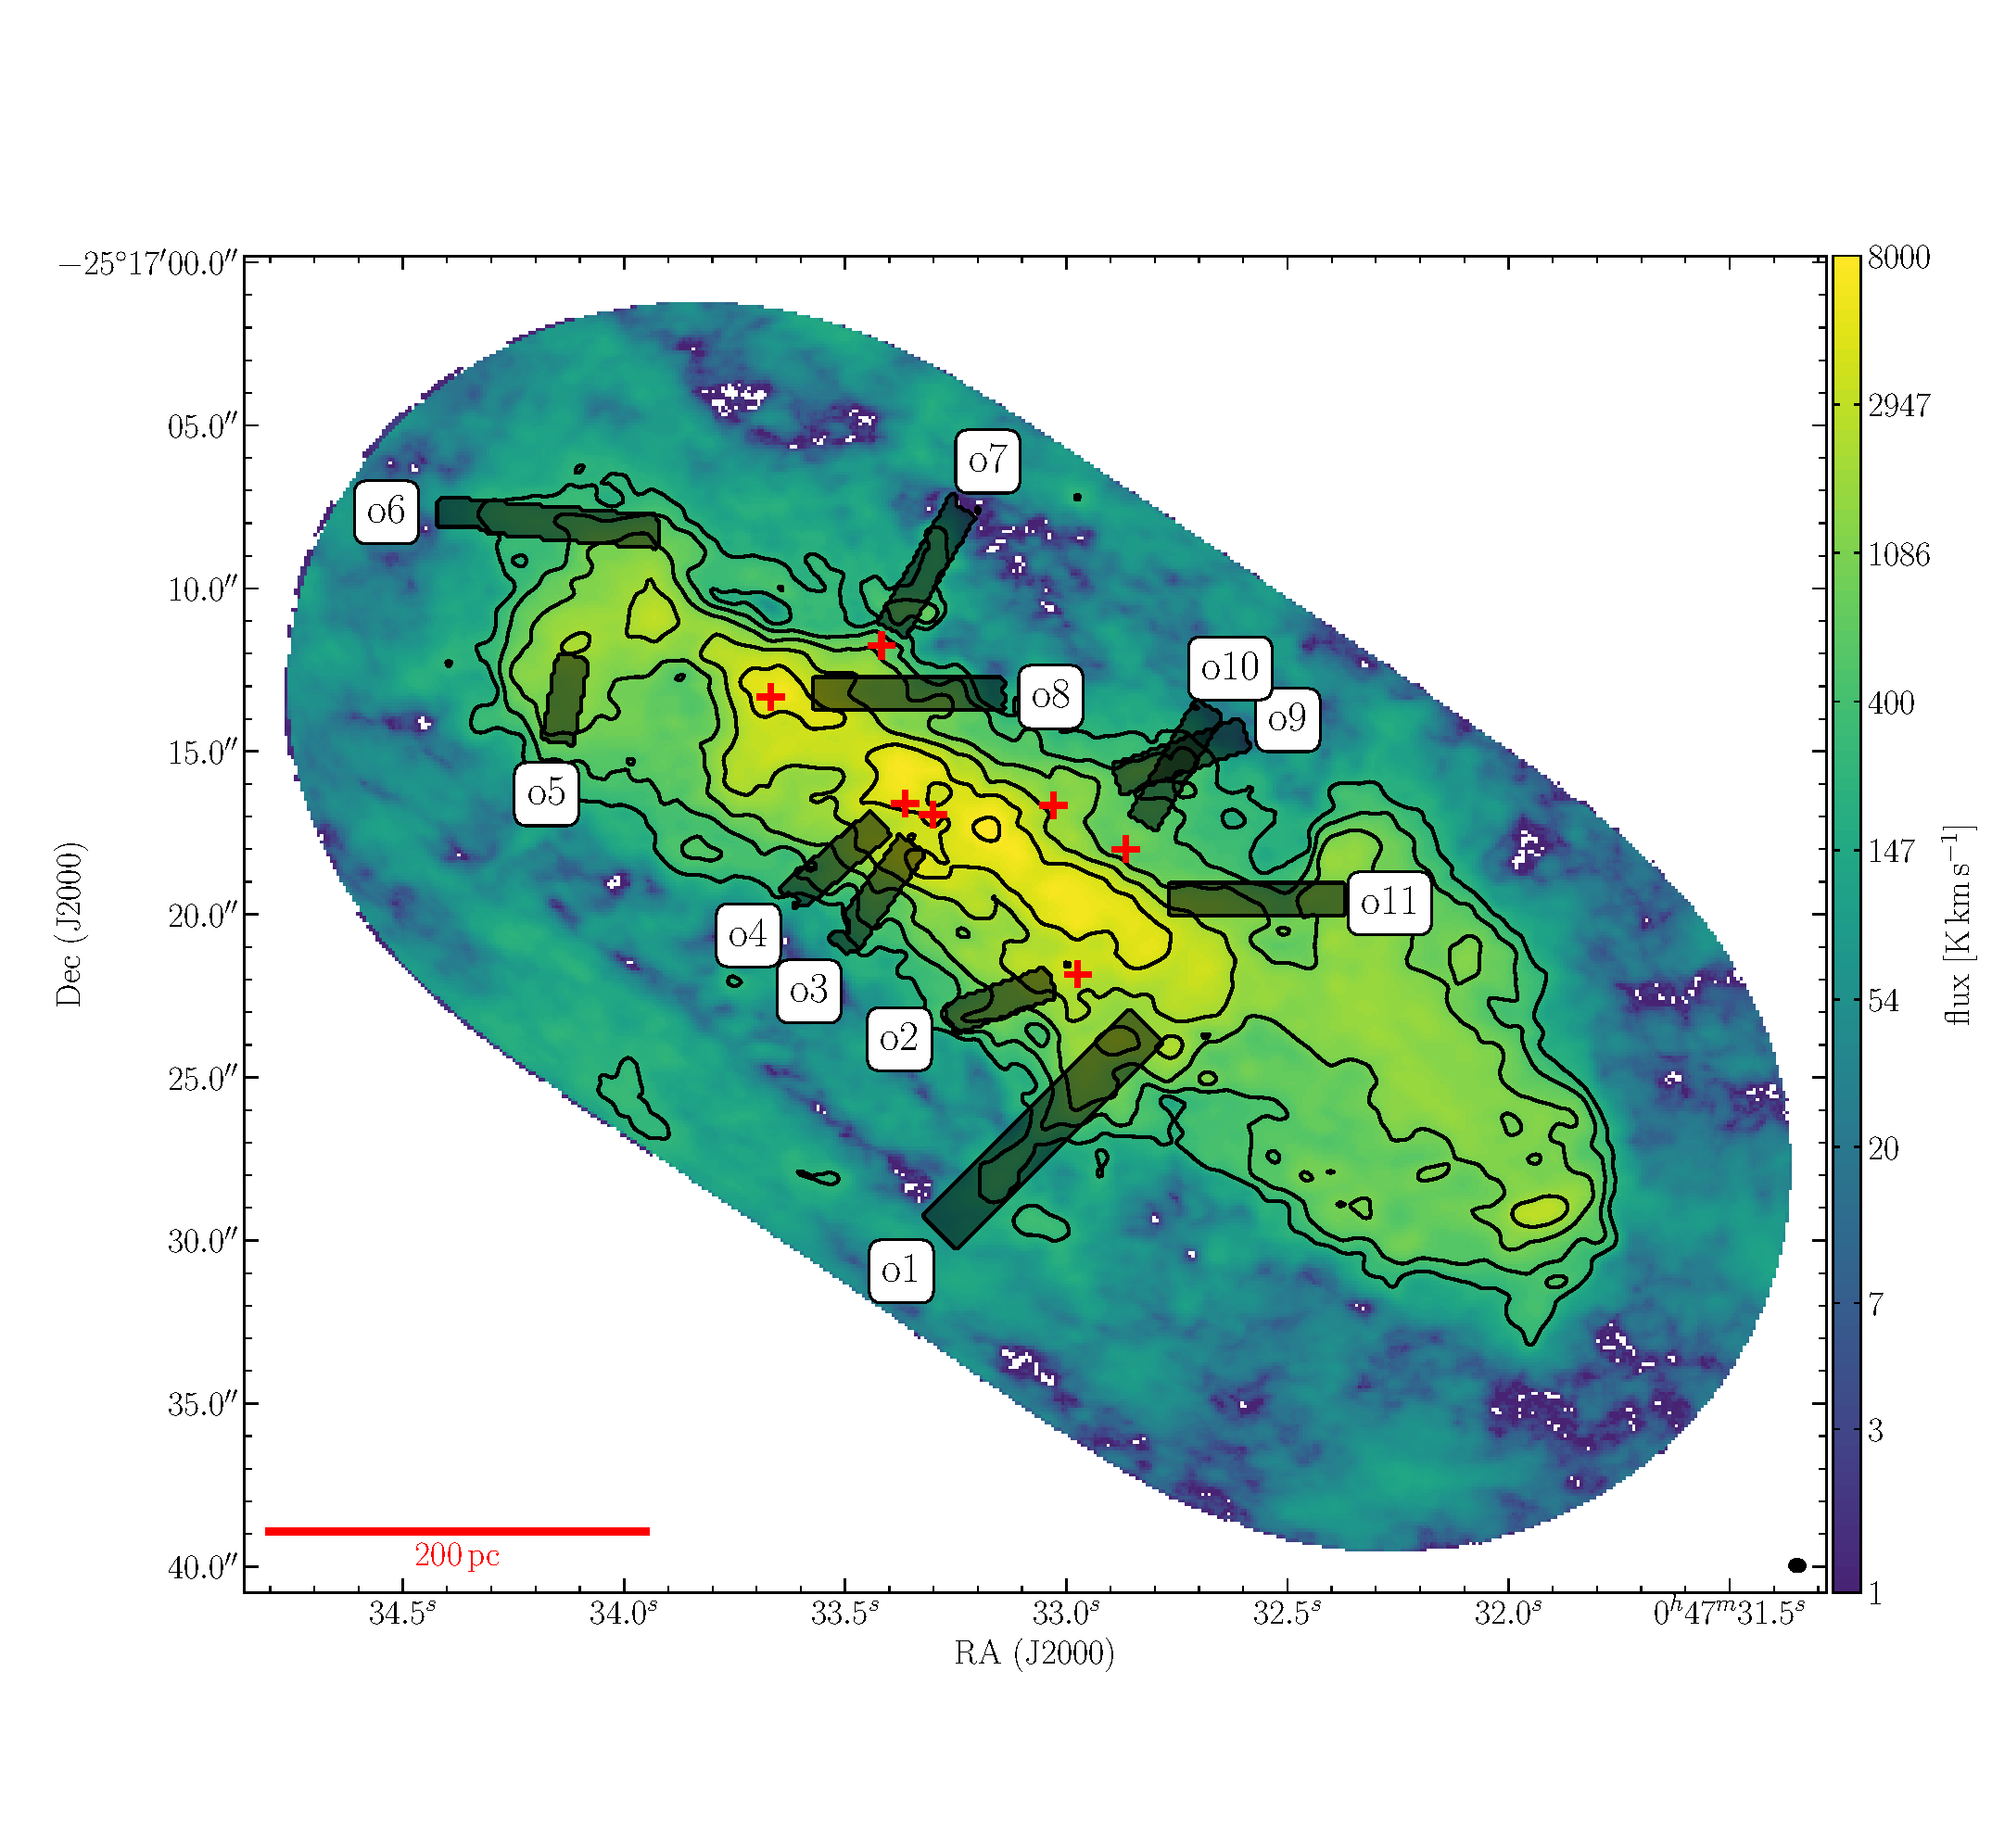
\includegraphics[width=\linewidth]{images/chapters/papers/outflow_catalog/fig7.pdf}
	\caption[Overview of identified small scale outflow candidates]{Positions of identified outflows as listed in Table~\ref{outflow catalog: table: outflow catalog}. The background shows the \co32 integrated intensity. Not all outflow candidates show up clearly in this map due to blending for fore-/background emission. However, they can be identified in position-velocity diagrams, which are calculated along each outflow (Figure~\ref{outflow catalog: figure: outflow catalog pV}) . The length of the overlaid boxes reflect the length over which the outflows can be traced in pV space. In the cases where the outflow can be traced back to the disk the potential launching sites are marked by red crosses.}
	\label{outflow catalog: figure: outflow catalog}
\end{figure}

\begin{figure}[p]
	\centering
	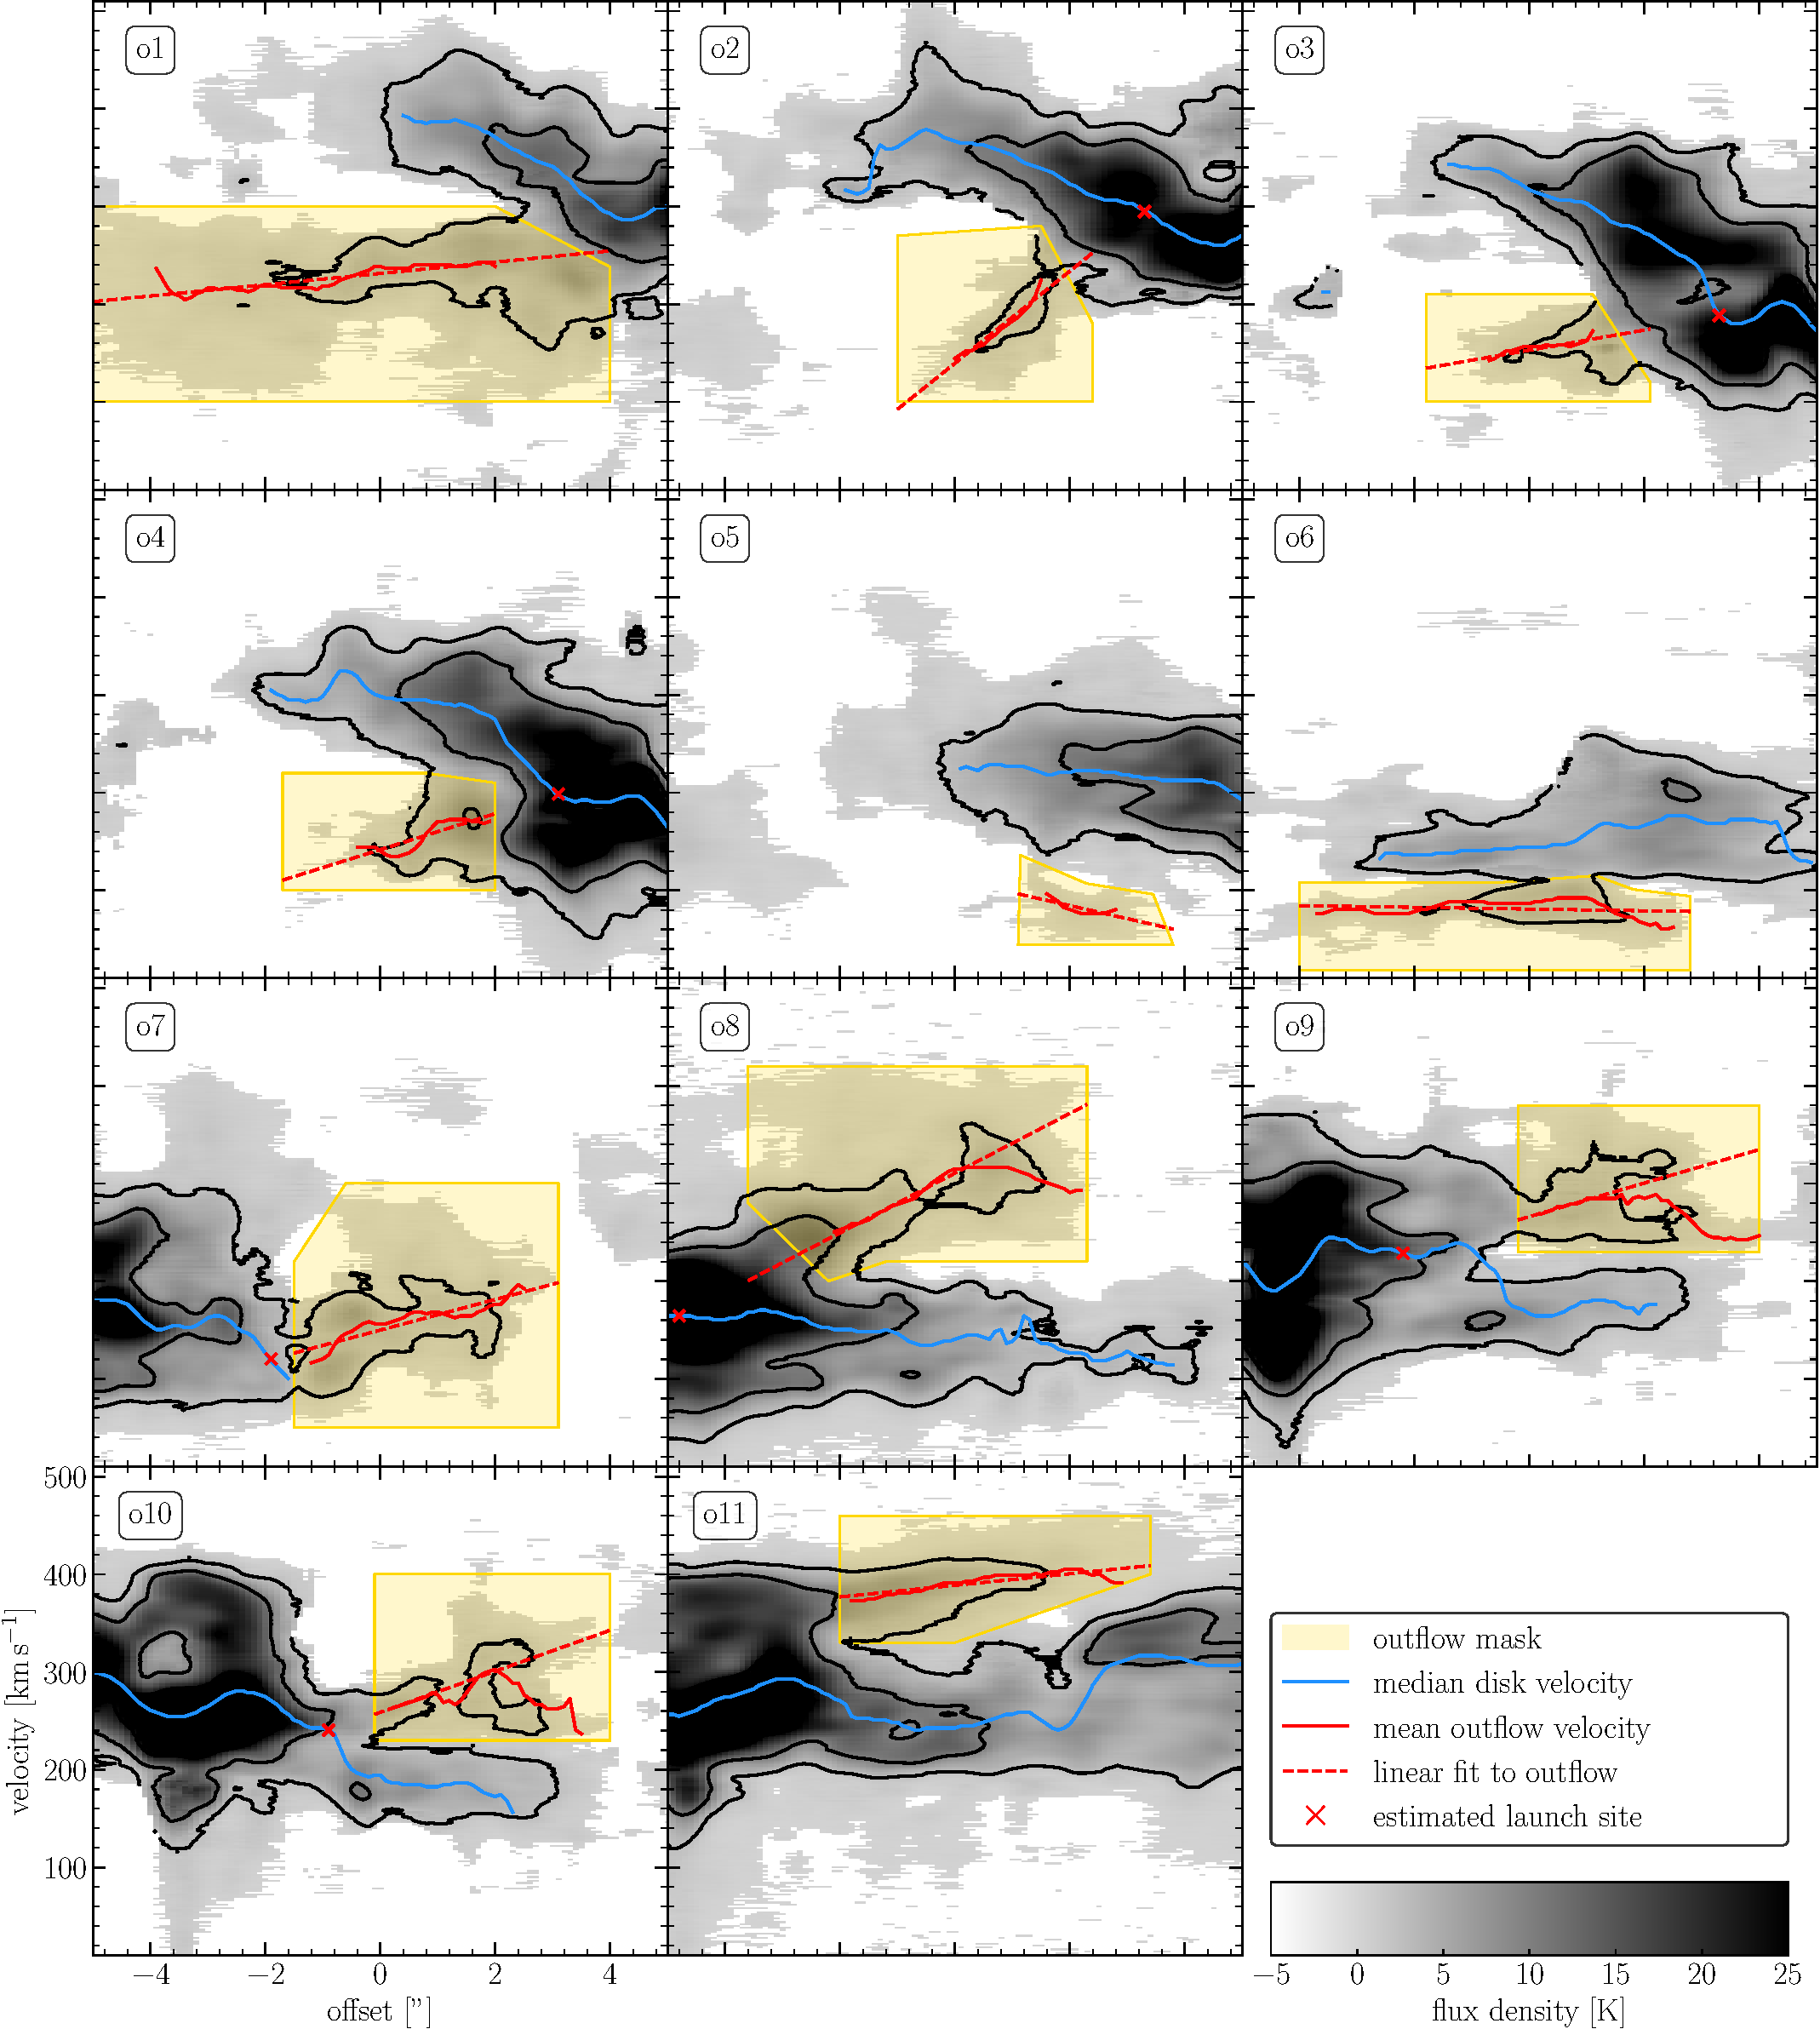
\includegraphics[width=\linewidth]{images/chapters/papers/outflow_catalog/fig8.pdf}
	\caption[Position-velocity diagrams of outflow candidates]{Position-velocity diagrams of the \co32 outflow candidates o1 to o11 masked at $5 \sigma$ (background grey scale images, saturated at 25\,K). The regions considered to be outflows is highlighted by golden outlines and shadings. Blue lines indicate the local median velocity of the molecular disk. Red lines indicate the local mean velocity in the outflow candidates that are fitted as indicated by dashed red lines. If the fitted outflow velocity gradient intersect the local disk, the intersection is marked by a red cross (o2, o3, o4, o7, o8, o9, o10).}
	\label{outflow catalog: figure: outflow catalog pV}
\end{figure}


%%%%%%%%%%%%%%%%%%%%%%%%%%%%%%%%%%%%%%%%%%%%%%%%%%%%%%%%%%%%%%%%%%%%%%%%%%%%%%%%%%%%%%%%%%%%%%%%%%%%
%%%%%%%%%%%%%%%%%%%%%%%%%%%%%%%%%%%%%%%%%%%%%%%%%%%%%%%%%%%%%%%%%%%%%%%%%%%%%%%%%%%%%%%%%%%%%%%%%%%%

\section{Outflow statistics}\label{outflow catalog: section: statistics}

Physical properties of the outflow candidates are listed in Table~\ref{outflow catalog: table: outflow catalog} and briefly discussed in the following.

\paragraph{Size}
The projected lengths of the outflow candidates range from 1.9\arcsec (32\,pc) to 11.0\arcsec (187\,pc) with a mean 4.9\arcsec (83\,pc). In all cases, the mean width is small $0.5"$ (8\,pc) to $1.4"$ (24\,pc) and close to the resolution limit.

\paragraph{Orientation}
Typically, the structures are oriented close to perpendicular to the plane of the star forming gas disk. The deviation from the minor axis is $\Delta\mathrm{PA} = 0^\circ - 35^\circ$ to the south and $\Delta\mathrm{PA} = 5^\circ - 55^\circ$ to the north.
Candidate o6 is almost parallel to the major axis and hence is unlikely to be an outflow driven by stellar feedback of the starburst.

\paragraph{Velocity range}
Derived velocity ranges over which the outflow candidates can be traced at the $5\sigma$-level are consistent for outflows on each side of the plane, $\sim 100-250$\,\kms to the south, $\sim 230-360$\,\kms to the north and thus symmetric to the systemic velocity of 250\,\kms.

\paragraph{Mass}
Individual mass estimates range between $5.31 \times 10^3$\,\Msun for the small o5 and $1.12 \times 10^6$\,\Msun for the large and massive SW streamer. The summed outflowing mass without o5 and o6 is $1.91\times 10^6$\,\Msun which is about a third of the lower limit found by \citet[][$6.6 \times 10^6$\,\Msun]{2013Natur.499..450B}. Such a fraction is reasonable given that this mass sums up only 9 distinctive features not considering less obvious features and diffuse outflows. 
The combined streamer masses amount to $\sim 5-10$\% of the total outflow mass in \co10 and \co21 in \citet[Chapter~\ref{chapter: outflow}]{2019ApJ...881...43K}. A more meaningful comparison is the \co32 outflow mass of $8.3 \times 10^6$ since the lower CO line observations cover significantly larger areas. Within $\sim 100$\,pc of the disk, the likely outflowing streamers (o1--o4, o7--o11) contribute $\sim 25$\% to the outflowing molecular gas mass. Adopting the proportion of $\sim 50$\% diffuse and $\sim 50$\% localized outflow as indicated in \citet[Chapter~\ref{chapter: outflow}]{2019ApJ...881...43K}, the streamer identified here make up already half of the localized outflowing \co32 mass.

\paragraph{Velocity gradient}
We find a wide variety of velocity gradients among the outflow candidates. All are accelerating with respect to the local disk velocity with the exception of o5 and o6 that are offset from but parallel to the disk velocity.
In the SW streamer (o1), the gradient is 0.34\,\kms\,pc$^{-1}$ which is almost identical to \citet[$0.36$\,\kms\,pc$^{-1}$]{2017ApJ...835..265W} who were able to trace this outflow further out in \co10.
Adopting their projection correction of a factor of $\sim 3$, our best estimate for the geometry corrected velocity gradient is 1.02\,\kms\,pc$^{-1}$, i.e. the molecular gas traced by \co32 is accelerating away from the disk.
Good estimates of the velocity gradients are obtained for o2 to o8 and o11, most of them accelerating faster than o1 at $0.36$\,\kms\,pc$^{-1}$ to $\sim 2.78$\,\kms\,pc$^{-1}$ in projection. Depending on the unknown geometry of each individual outflow candidate, the 3D velocity gradient can be greater by factors of unity to a few.
Gradients of the other candidates need special discussion as they are affected by several effects.
In both o9 and o10, the proposed outflow splits into two parts that are at constant velocity and accelerating at $\GTRSIM 1.0$\,\kms\,pc$^{-1}$ which is not well reflected by a combined fit.
The origin of the splitting cannot be inferred from the data at hand and must be addressed in a more detailed study.
The velocity of o5 and o6 is oriented parallel to that of the disk, so they cannot be considered outflows but rather a second kinematic component, e.g. a foreground cloud.

\paragraph{Launching sites}
The projected launching sites defined by tracing back the velocity gradient to the disk lie close to the star forming disk midplane for o3, o4 and o8.
Furthermore, the launching sites of o2, o3, o4, o9 and o10 can be considered close (offset $\LESSSIM 1\arcsec$ or $\LESSSIM 20$\,pc) to sites of recent star formation in star forming massive clumps \citep{2017ApJ...849...81A} and (proto-) SSCs \citep{2018ApJ...869..126L}.
Note that the positional accuracy of the launching site estimation depends strongly on the velocity gradient and is $0.5\arcsec-1.0\arcsec$. Furthermore, the back-traced launching sites are projected positions and do not necessarily lie close to the clumps and SSCs in 3D space. The inferred proximity, however, is reassuring.
The SSCs currently undergoing star formation are most likely not the launching sites of the observed outflows because of feedback delay. The amount of time required to form the observed outflows (kinematic ages $\sim$ Myr, see below) and the time delay until the first supernovae explode after the onset of star formation (several Myr) is older than the age of the (proto-)SSCs. Recently, \citet{2020MNRAS.491.4573R} age-dated half of the 14 (proto-)SSCs in \ngc253 to $\LESSSIM 1$\,Myr while the other half is still on the zero-age main sequence and thus also still very young. 
The outflow candidate launching site are then not expected to match exactly the locations of current clusters. Older clusters that might have launched the observed outflow candidates should have formed at similar locations within the disk. An approximate correspondence between sites of on-going star formation and the launching sites is therefore expected.

\paragraph{Velocity dispersion}
Velocity dispersions within the outflow candidates vary by a factor of $\sim 2$ across the candidates with the highest dispersions of $\GTR 30$\,\kms found in the most massive outflows o1, o7 and o8.
The low dispersions of $\sim 13$\,\kms in o5 and o6 support the idea that these are of different origin than the other outflow candidates.
\citet{2017ApJ...835..265W} state a somewhat wider $35 - 40$\,\kms for the SW streamer (o1) in \co10 than the 34.1\,\kms that we find in \co32 which is potentially due to the higher excitation state.

\paragraph{Kinetic energy}
The internal kinetic energy derived from the velocity dispersion $E_\mathrm{kin,disp}$ is typically a few times $10^{49}$\,erg. o2 and o3 are significantly less energized owing to their low mass. Due to their low velocity dispersion, o5 and o6 also contain low amounts of internal kinetic energy.

The bulk kinetic energy of an outflow $\mathrm{E}_{kin,launch}$ can be calculated only for the candidates for which a launching site can be estimated and varies strongly between $\sim 6 \times 10^{48}$\,erg (o3) and $\GTR  5 \times 10^{50}$\,erg (o8).
The very high energy in o8 is explained by being massive and having a strong velocity gradient; the line-of-sight velocity at its tip is $\sim 160$\,\kms faster than at the estimated launching point.

Comparing the two energy estimates, o2 and o8 are dominated by bulk kinetic energy with $E_\mathrm{kin,launch} \GTRSIM 10 \times E_\mathrm{kin,disp}$.
In the other cases where both energies could be calculated, $E_\mathrm{kin,disp} \simeq E_\mathrm{kin,launch}$ to a surprising precision of a factor $\LESS 2-3$.
This results argues for approximate energy partition between internal and bulk kinetic energy in a typical molecular streamer.

\paragraph{Dynamical age}
For o5 and o6, no meaningful dynamical age can be calculated because their velocity gradients are close to parallel to the local disk velocity.
For the other candidates, the short ages of $\sim 1.2$\,Myr on average indicate that the observed molecular streamers are mostly a young feature.
o1 and o11, however, are significantly older with 3.0 and 2.5\,Myr, respectively.

For o1, \citet{2017ApJ...835..265W} report an age of $\sim 1$\,Myr with a projection correction factor of $\sim 3$ as given by \citet{2013Natur.499..450B}.
Our assumption of a perpendicular outflow translates to a projection correction of $\left[ \sin \left( i-90^\circ \right) \right]^{-1} \sim 5$.
If we also adopt a projection correction of 3 instead of 5, the dynamical age of o1 would be 1.8\,Myr instead of 3.0\,Myr.

We expect age uncertainties of a factor of at least $\sim 2$ due to the unknown geometry alone. A factor of two translates to a deviation from perpendicular orientation by just $\sim 10^\circ$. Even when considering this uncertainty, the molecular outflow candidates are kinematically young features and likely all younger than a few Myr.

\begin{sidewaystable}
% \begin{table}
	\centering
% 	\tablewidth{\textwidth}
    \begin{threeparttable}
	    \caption[Catalog of outflow features]{Catalog of the outflows indicated in Figure~\ref{outflow catalog: figure: outflow catalog}.
	        \label{outflow catalog: table: outflow catalog}}
%	    \vspace{}
    \begin{tabular}{cccccccccccc}
        \toprule
        \multirow{2}{*}{name} & mid point: RA, DEC & length\tnote{a} & width\tnote{a} & PA\tnote{b} & velocity\tnote{c} & mass\tnote{d} & gradient\tnote{e} & dispersion\tnote{f} & E$_{kin,disp}$\tnote{g} & E$_{kin,launch}$\tnote{h} & t$_{dyn}$\tnote{i}\\
		& (J2000) & ["] & ["] & [$^\circ$] & [km\,s$^{-1}$] & [\Msun] & [km\,s$^{-1}$\,pc$^{-1}$] & [km\,s$^{-1}$] & [erg] & [erg] & [Myr]\\
        \midrule
    	o1  & 00:47:33.034, -25:17:26.352 & 11.0 & 1.1 & 135 & 180-250 & $1.12 \times 10^6$ & 0.34  & 34.1 & $5.05 \times 10^{49}$ & & 3.0\\
	    o2  & 00:47:33.204, -25:17:22.970 & 2.8  & 0.9 & 110 & 100-200 & $3.21 \times 10^4$ & 2.78  & 21.8 & $6.65 \times 10^{48}$ & $1.16 \times 10^{50}$ & 0.3\\
	    o3  & 00:47:33.442, -25:17:19.660 & 3.0  & 0.8 & 145 & 126-174 & $3.99 \times 10^4$ & 0.61  & 16.8 & $2.11 \times 10^{48}$ & $6.01 \times 10^{48}$ & 1.5\\
	    o4  & 00:47:33.538, -25:17:18.581 & 2.6  & 0.5 & 130 & 120-160 & $7.61 \times 10^4$ & 1.09  & 18.6 & $1.23 \times 10^{49}$ & $3.01 \times 10^{49}$ & 0.8\\
	    o5  & 00:47:34.170, -25:17:15.919 & 1.9  & 0.9 & 170 & 180-250 & $5.31 \times 10^3$ & -0.78 & 12.7 & $3.61 \times 10^{47}$ & & \\
	    o6  & 00:47:34.133, -25:17:08.148 & 7.1  & 1.4 & 85  & 60-170  & $9.64 \times 10^4$ & -0.04 & 13.3 & $3.44 \times 10^{48}$ & & \\
	    o7  & 00:47:33.347, -25:17:10.091 & 4.2  & 1.1 & 330 & 80-230  & $1.22 \times 10^5$ & 0.91  & 34.4 & $4.25 \times 10^{49}$ & $4.47 \times 10^{49}$ & 1.0\\
	    o8  & 00:47:33.315, -25:17:13.329 & 5.2  & 0.8 & 270 & 260-360 & $2.57 \times 10^5$ & 1.80  & 32.6 & $4.63 \times 10^{49}$ & $5.40 \times 10^{50}$ & 0.5\\
	    o9  & 00:47:32.880, -25:17:15.919 & 2.9  & 1.1 & 290 & 230-350 & $7.69 \times 10^4$ & 1.03  & 25.9 & $2.29 \times 10^{49}$ & $6.33 \times 10^{49}$ & 0.9\\
	    o10 & 00:47:32.832, -25:17:17.214 & 4.1  & 1.2 & 330 & 240-300 & $6.02 \times 10^4$ & 1.22  & 28.9 & $1.38 \times 10^{49}$ & $2.68 \times 10^{49}$ & 0.7\\
	    o11 & 00:47:32.630, -25:17:19.660 & 4.5  & 0.8 & 270 & 260-330 & $1.25 \times 10^5$ & 0.36  & 19.0 & $1.04 \times 10^{49}$ & & 2.5\\
	    \midrule
	    mean/sum$^j$ &                    & 4.9  & 1.0 &     &         & $1.90 \times 10^6$ & 1.13  & 25.7 & $2.31 \times 10^{49}$ & $1.09 \times 10^{50}$ & 1.2\\
        \bottomrule
    \end{tabular}
    \vspace{0.5em}
	\begin{tablenotes}
		\item[a] projected range over which the outflow can be traced in the channel maps at the $5 \sigma$ level
		\item[b] north to east
		\item[c] velocity range in which the outflow can be traced in the channel maps at the $5 \sigma$ level
		\item[d] H$_2$ mass assuming a starburst $\mathrm{X}_{CO} = 0.5 \times 10^{20}$\,\sqcm
		\item[e] velocity gradient along the outflow
		\item[f] mean dispersion per channel
		\item[g] kinetic energy derived from velocity dispersion
		\item[h] kinetic energy relative to the launching site
		\item[i] dynamical age of the outflow tip
		\item[j] without o5 and o6 which are considered not to be outflows (see text); for the mass, the sum instead of the mean is given
	\end{tablenotes}
	\end{threeparttable}
% \end{table}
\end{sidewaystable}

%%%%%%%%%%%%%%%%%%%%%%%%%%%%%%%%%%%%%%%%%%%%%%%%%%%%%%%%%%%%%%%%%%%%%%%%%%%%%%%%%%%%%%%%%%%%%%%%%%%%
%%%%%%%%%%%%%%%%%%%%%%%%%%%%%%%%%%%%%%%%%%%%%%%%%%%%%%%%%%%%%%%%%%%%%%%%%%%%%%%%%%%%%%%%%%%%%%%%%%%%

\section{Discussion}

The high resolution achievable with ALMA allows to detect a surprising level of substructure around the starburst in \ngc253. The previously highest resolution study in \citet[32\,pc spatial resolution]{2017ApJ...835..265W} could detect only the SW streamer as a localized feature close to the resolution limit.
The sample of molecular streamers in this work allows us to infer the typical properties and variations thereof. Although on a small statistical basis, trends can be inferred.

The kinetic and structural parameters of the 11 outflow candidates reveals that most of them indeed show evidence of being driven out from the starburst by feedback. Candidates o5 and o6 are likely not outflowing but other molecular clouds that do not kinematically match the disk and exhibit a high aspect ratio. Their location at the edge of the molecular disk towards the bar indicate that they could potentially be infalling molecular clouds. Due to the high inclination of \ngc253, o5 and o6 can also be fore-/background clouds off the midplane in the spiral arms.

The other candidates o1-o4 and o7-o11 are likely to be outflowing molecular structures. Their projected geometry and velocity structure are consistent with individual molecular clouds flowing away from a launching site in the disk while getting dispersed along the flow direction.
For o1 (SW streamer), the only streamer described before, our measurements match closely to the literature values. For the other outflowing streamers, we obtain plausible results lower than for o1, the most massive and largest streamer.

The formation of outflowing streamers is unclear and cannot be inferred from our analysis. Now that they are characterized, potential formation scenarios can be tested.
Each molecular streamer could be an independent collimated feature. The collimation of the outflowing gas down to $\leq 20$\,pc in this scenario is unclear. A potential collimation mechanisms may be the entrainment of molecular gas in an ionized flow after (super-)bubble breakout. Over-pressurized, ionized gas due to feedback is known to vent through channels of least resistance in the disk \citep[e.g.][]{2012ApJ...760..155K,2016MNRAS.456.3432G} that could entrain molecular gas. In that case, the streamers are the extension of feedback vents. 
More likely, however, is a scenario in which a large stratified outflow fragments. The multi-phase outflow cone in \ngc253 is thought to be radially stratified \citep[as shown in Figure~\ref{introduction: figure: star formation: outflow cone}]{2015ApJ...801...63M} with a thin shell of molecular gas surrounding the ionized outflow. Such a thin sheet of dense gas is unlikely to remain stable even on short timescales, but expected to fragment. The outflow cone would then break up into a set of narrow dense streamers. The remaining molecular gas in between the streamer might accrete locally onto the streamers or get dissociated/ionized quickly due to diminishing self-shielding against the adjacent ionized outflow.
Specialized, parsec scale resolution simulations and observations across all outflow gas phases will be required to reveal potential interactions.


%%%%%%%%%%%%%%%%%%%%%%%%%%%%%%%%%%%%%%%%%%%%%%%%%%%%%%%%%%%%%%%%%%%%%%%%%%%%%%%%%%%%%%%%%%%%%%%%%%%%
%%%%%%%%%%%%%%%%%%%%%%%%%%%%%%%%%%%%%%%%%%%%%%%%%%%%%%%%%%%%%%%%%%%%%%%%%%%%%%%%%%%%%%%%%%%%%%%%%%%%


\section{Summary}

We follow up the global look at the \ngc253 starburst outflow by a high-resolution look at individual, potentially outflowing, structures in \co32 that we refer to as streamers.
We identify eleven distinct features by eye, nine of which are kinematically consistent with being outflows and two potentially infalling GMCs.

\begin{enumerate}[noitemsep,topsep=0pt]

\item The outflows are close to perpendicular to the gas disk with mean projected sizes of $4.9\arcsec \times 1.0\arcsec$ ($83\,\mathrm{pc} \times 17\,\mathrm{pc}$).

\item The combined mass of the nine outflows is $1.9 \times 10^6$\,\Msun, about half of the mass in localized outflows found in \co32 in \citet[, Chapter~\ref{chapter: outflow}]{2019ApJ...881...43K}.
The outflows are accelerating away from the disk with a mean velocity gradient of 1.13\,\kms\,pc without projection correction.

\item By tracing back the outflow candidates to the disk, we are able to estimate the launching sites and find them to lie close to the major axis of the molecular disk and in five cases also close (offset $\sim 1\arcsec$ or $\sim 20$\,pc) to sites of current cluster formation.

\item Within the streamers, the mean velocity dispersion is $\sim 26$\,\kms which results in a typical turbulent energy of a few $10^{49}$\,erg.
If a launching site could be estimated, the bulk kinetic energy is typically a few times $10^{49}$\,erg but an order of magnitude higher for two streamers with particularly steep velocity gradients.
This result implies that streamers are typically in approximate energy equipartition between internal and bulk kinetic energy.

\item All streamers are kinematically young $\leq 3$\,Myr and typically $\sim 1$\,Myr old.

\end{enumerate}

Further high-resolution observations across the gas phases and simulations are required to reveal the formation mechanism of outflowing streamers.